\documentclass[a4paper,10pt]{article}
\usepackage[english]{babel}
\usepackage[utf8]{inputenc}
%Includes "References" in the table of contents
\usepackage[nottoc]{tocbibind}
\usepackage{url}
\usepackage{graphicx}
\usepackage{hyperref}


%Title, date an author of the document
\title{Weekly Update}
\author{Khalimat Murtazalieva}

%Begining of the document
\begin{document}

\maketitle

\tableofcontents

\medskip


\section{Task № 1}
\subsection{Description}
Perform the same comparison as you have done for AL and non\_AL by including the other down-sampling or up-sampling methods you have suggested, so we can see whether AL would also perform better than other sampling technologies.

\subsection{Solution}
I have chosen three sampling strategies you outlined in \href{https://github.com/Khalimat/SCAMmer}{README}:
\begin{itemize}
    \item \href{https://imbalanced-learn.readthedocs.io/en/stable/generated/imblearn.over_sampling.ADASYN.html}{ADASYN}
    \item \href{https://imbalanced-learn.readthedocs.io/en/stable/generated/imblearn.over_sampling.SMOTE.html}{SMOTE}
    \item \href{https://imbalanced-learn.readthedocs.io/en/stable/generated/imblearn.under_sampling.CondensedNearestNeighbour.html}{CondensedNearestNeighbor}
\end{itemize}

I compared every sampling strategy from the list above with \href{https://modal-python.readthedocs.io/en/latest/content/apireference/uncertainty.html}{uncertainty sampling} from modAL (run 10 fold cross validation and calculated t-test stats for AUC lower boundary, AUC, AUC upper boundary, accuracy, F1, MCC). 

All performance metrics for models trained using uncertainty sampling are significantly higher than for models trained using SMOTE. Please see Figure~\ref{fig:2} for screenshot with stats (also, see table "t-test stats.csv" in "./results/SMOTE")

All performance metrics for models trained using uncertainty sampling are significantly higher than for models trained using ADASYN except for F1 (0.533 ADASYN vs. 0.566 uncertainty sampling, but difference is not statistically significant). Please see Figure~\ref{fig:3} for screenshot with stats (also, see table "t-test stats.csv" in "./results/ADASYN")

All performance metrics for models trained using uncertainty\_sampling are significantly higher than for models trained using CondensedNearestNeighbour except for F1 (0.567 CondensedNearestNeighbour vs. 0.565 uncertainty sampling). Please see Figure~\ref{fig:4} for screenshot with stats (also, see table "t-test\_stats.csv" in "./results/CondensedNearestNeighbour")


\section{Task № 2}
\subsection{Description}
Include other ML methods and other AL sampling methods
\subsection{Solution}
I wrote in one of the previous email that uncertainty sampling could work only with ensemble models, of course it is not correct, it works with any probabilistic model, as we just need to find samples nearest to the decision boundary.

\section{Task № 3}
\subsection{Description}
Try pipeline on the different datasets for SCAMs
\subsection{Solution}

\section{Task № 4}


\subsection{Description}
Revisit the scaffold-based train/test splitting to generate more difficult machine learning problems.
\subsection{Solution}
I decided to implement \href{https://www.rdkit.org/docs/source/rdkit.ML.Cluster.Butina.html}{RDKit butina clustering algorithm}\cite{butina1999unsupervised}, since \href{https://imbalanced-learn.org/stable/install.html}{I need scikit-learn 0.23 in environment to run imbalanced-learn}, but current deepchem version is incompatible with scikit-learn 0.23 \href{https://github.com/deepchem/deepchem/issues/1861}{(see. issue here, Bharath kindly informed me that I can use nightly build, but I have already implemented functions based on butina clustering)}. The current version of butina split include in the test set only molecules which are "lonely" in their clusters, so we preclude the case when training set include many molecules that are very similar to the ones in the test set (I used function written by Patrick Walters to generate clusters, please, see butina\_cluster in utilities.py and wrote a function split\_with\_butina in main.py). I run 10-fold cross-validation with butina splitter and compared AL- non-AL models performance using paired t-test (see Fig.~\ref{fig:1}). We observe that model trained using AL strategy perform better based on all metrics. Also, see table "t-test\_stats.csv" in "./results/Butina".



\begin{figure}[1]
    \centering
    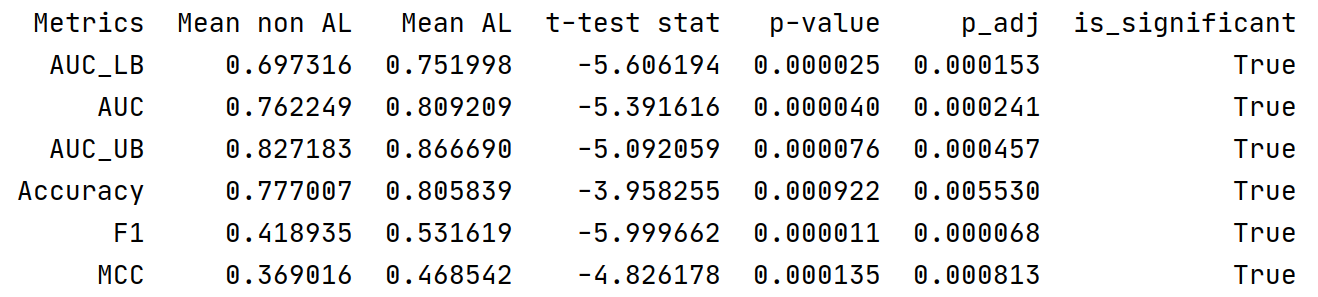
\includegraphics[keepaspectratio=true, scale=0.33]{images/Butina.png}
    \caption{AL and non-AL models performance comparison. Butina splitter}
    \label{fig:1}
\end{figure}

\begin{figure}[2]
    \centering
    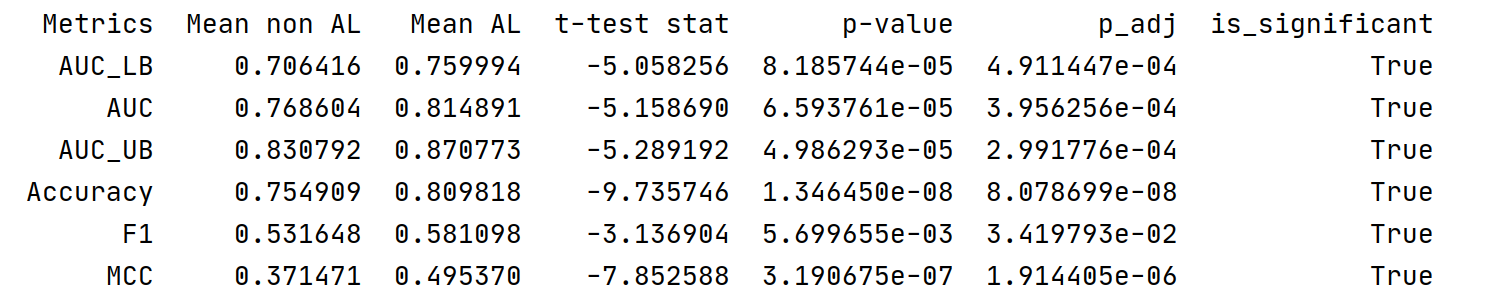
\includegraphics[keepaspectratio=true, scale=0.31]{images/SMOTE_1.png}
    \caption{AL and non-AL (SMOTE sampling) models performance comparison. Random splitter}
    \label{fig:2}
\end{figure}

\begin{figure}[3]
    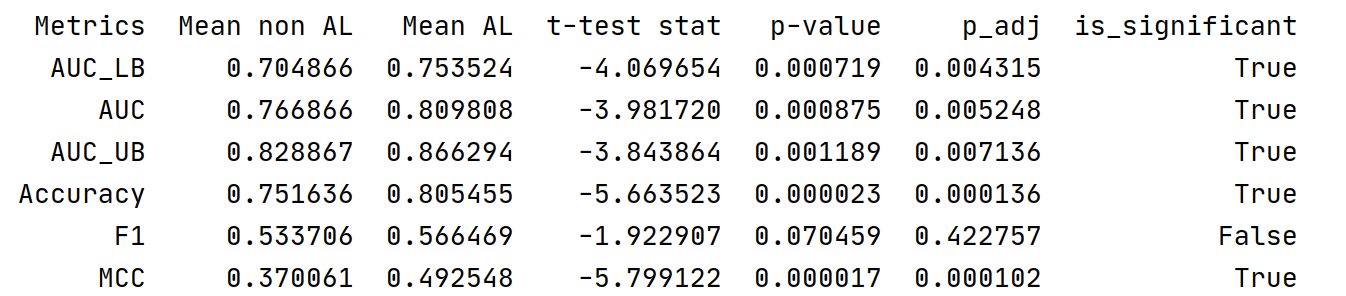
\includegraphics[keepaspectratio=true, scale=0.33]{images/ADASYN.png}
    \caption{AL and non-AL (ADASYN sampling) models performance comparison. Random splitter}
    \label{fig:3}
\end{figure}

\begin{figure}[4]
    \centering
    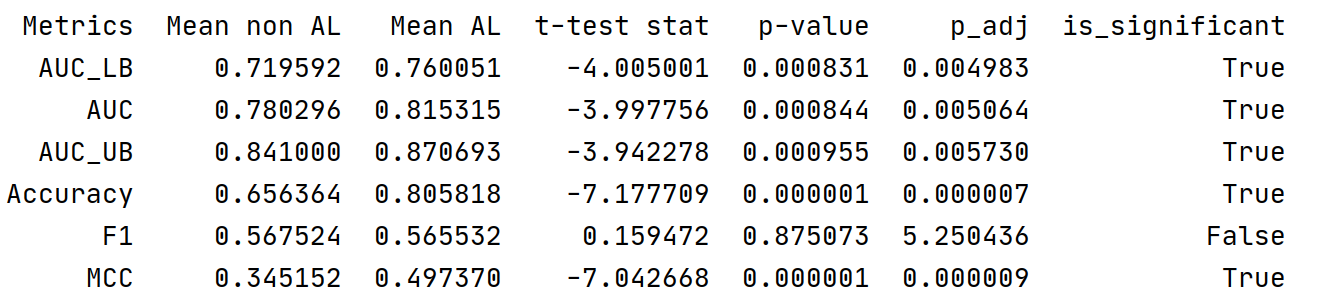
\includegraphics[keepaspectratio=true, scale=0.33]{images/CondensedNearestNeighbour.png}
    \caption{AL and non-AL (CondensedNearestNeighbour sampling) models performance comparison. Random splitter}
    \label{fig:4}
\end{figure}


\begin{figure}[5]
    \centering
    \includegraphics[keepaspectratio=true, scale=0.32]{images/Metrics.png}
    \caption{Performance of models trained using Uncertainty Sampling (US) or other sampling approaches}
    \label{fig:5}
\end{figure}

\medskip

%Sets the bibliography style to UNSRT and imports the 
%bibliography file "samples.bib".
\bibliographystyle{unsrt}
\bibliography{sample}

\end{document}
